% =====================================================================
% Medi-Script-AI: A Hybrid Deep Learning Pipeline for Structured
% Information Extraction from Handwritten Medical Prescriptions
%
% Template: IEEEtran (conference), the standard two-column CS/ML
% systems-paper template.
% =====================================================================
\documentclass[conference]{IEEEtran}

\usepackage{graphicx}
\usepackage{amsmath}
\usepackage{booktabs}
\usepackage{microtype}
\usepackage{cite}
\usepackage{xcolor}
\usepackage{listings}
\usepackage{subcaption}
\usepackage[hidelinks]{hyperref}

% ---- lightweight, monospace "record / log" box -----------------------
\definecolor{codebg}{RGB}{245,246,248}
\definecolor{coderule}{RGB}{210,214,220}
\lstdefinestyle{recordbox}{
  backgroundcolor=\color{codebg},
  basicstyle=\ttfamily\small,
  breaklines=true,
  frame=single,
  rulecolor=\color{coderule},
  framesep=6pt,
  xleftmargin=2pt,
  xrightmargin=2pt,
  columns=flexible,
}
\lstset{style=recordbox}

\begin{document}

% ---------------------------------------------------------------------
% TODO (author): replace the placeholder name / affiliation / email
% below before submission.
% ---------------------------------------------------------------------
\title{Medi-Script-AI: A Hybrid Deep Learning Pipeline for Structured\\
Information Extraction from Handwritten Medical Prescriptions}

\author{
  \IEEEauthorblockN{Author Name(s) To Be Added}
  \IEEEauthorblockA{
    Department / Affiliation To Be Added\\
    Email: author@example.edu
  }
}

\maketitle

\begin{abstract}
Handwritten medical prescriptions remain a critical bottleneck in the digital transformation of healthcare: illegible handwriting and manual transcription contribute to thousands of preventable medication errors each year, with the extra medical costs of drug-related injuries in U.S.\ hospitals alone estimated at \$3.5 billion annually. This paper presents \textbf{Medi-Script-AI}, a two-stage pipeline that separates prescription digitization into \emph{field localization} -- a custom fine-tuned YOLOv8-nano detector -- and \emph{handwriting recognition} -- a Transformer-based OCR model (TrOCR), cross-checked against EasyOCR and corrected against a 1{,}142-entry medical lexicon -- to produce a structured JSON record of patient and clinical fields. Unlike document-understanding transformers that treat a prescription as a generic layout, we treat localization and recognition as separable problems best solved by two specialist models, and we report results for both honestly and separately. Our fine-tuned detector reaches \textbf{86.1\% mAP50} (46.2\% mAP50-95, 81.9\% precision, 80.6\% recall) on a real-world, single-class prescription benchmark, training in under five minutes on a single GPU -- showing that reliable field localization is achievable even from a small, imperfectly annotated dataset. Pairing this detector with an \emph{off-the-shelf} handwriting-recognition model does not yet yield a working end-to-end system, however: we present a qualitative error analysis showing that pretrained TrOCR, without domain fine-tuning, produces either low-confidence noise or fluent, high-confidence hallucinations on real doctors' handwriting, and that our lexicon-based confidence gate correctly suppresses these errors rather than emitting a wrong answer. We contrast this with a synthetic-data-trained Donut baseline, which fails even more completely on the same class of images. Together, these results localize the true bottleneck in prescription digitization to handwriting recognition rather than field detection, and motivate a concrete, already-scoped fine-tuning plan as the next step toward a deployable system.
\end{abstract}

\begin{IEEEkeywords}
handwritten text recognition, medical prescription digitization, object detection, YOLOv8, TrOCR, document understanding, healthcare informatics
\end{IEEEkeywords}

% =====================================================================
\section{Introduction}
\label{sec:intro}

Medical prescriptions serve as the primary interface between a physician's clinical decision and a patient's treatment. In many parts of South Asia and across the developing world, however, prescriptions are still handwritten, often on printed hospital pads with irregular layouts. A report by the Institute of Medicine estimated that medication errors harm at least 1.5 million people every year in the United States, and that the extra medical costs of treating drug-related injuries in hospitals alone reach at least \$3.5 billion a year~\cite{iom2007medicationerrors}; a significant proportion of these errors are attributed to illegible handwriting or transcription mistakes during dispensing.

The manual digitization of these documents -- where a pharmacist or data-entry operator reads and types out each field -- is slow and error-prone. A system that can reliably and automatically convert a photograph of a handwritten prescription into a structured, machine-readable record would reduce:
\begin{itemize}
  \item \textbf{Dispensing errors} caused by illegible drug names or dosages.
  \item \textbf{Administrative overhead} in hospitals and clinics.
  \item \textbf{Barriers to patient health-record integration} in Electronic Medical Record (EMR) systems.
\end{itemize}

The core challenge is that this is not a generic document-digitization problem. A prescription is a semantically structured artifact where different \emph{regions} of the document carry different \emph{types} of information (name, age, medicine, dosage), and the handwriting within those regions is highly variable across practitioners. A solution must therefore address two distinct problems simultaneously: \emph{where} is the information, and \emph{what} does it say.

Formally, given a single RGB photograph of a handwritten prescription $P$, our objective is to extract a structured record $R$:

\begin{lstlisting}
R = {
  patient: { name, age, gender },
  clinical: { symptoms, prescription, dosage }
}
\end{lstlisting}
\label{sec:record}

where each field in $R$ is extracted directly from the corresponding visual region of $P$ -- not inferred or hallucinated. This is complicated in practice by arbitrary, non-standardized prescription-pad layouts; severe handwriting-style variability between practitioners; visually ambiguous corrections and abbreviations; and domain vocabulary -- drug names such as \emph{Pantoprazole} and \emph{Gliclazide} -- that is out-of-vocabulary for generic language models. \S\ref{sec:challenges} discusses these and further data- and deployment-level challenges in detail. The system must also return a result fast enough for clinical use, which rules out multi-model ensemble approaches with redundant forward passes (\S\ref{sec:temporal-coupling}).

This paper introduces \textbf{Medi-Script-AI}, a system that addresses both problems in sequence with a purpose-built hybrid pipeline. Rather than presenting only the metrics that flatter the system, we report our field-localization results alongside a detailed, evidence-based account of where and why the current recognition stage still fails on real handwriting -- because, at this stage of the project, that failure analysis is as informative as the numbers that work.

% =====================================================================
\section{Related Work}
\label{sec:related}

\subsection{Rule-Based and Template-Matching Systems}

Early systems for prescription digitization relied on fixed templates and OCR with predefined zone boundaries (e.g., ``the medicine field is always in columns 2--8, rows 10--14''). These worked reliably only when the prescription-pad layout was fixed and known in advance. They break completely when a new hospital's pad is introduced, cannot handle handwriting that bleeds outside the predefined zone, and do not generalize to unseen layouts.

\subsection{Generic OCR Followed by NLP Post-Processing}
\label{sec:generic-ocr}

A common modern approach runs a commercial OCR engine (e.g., Google Cloud Vision, AWS Textract, Tesseract) on the entire prescription image to extract a flat text string, then applies Named Entity Recognition (NER) or rule-based parsing to identify medicine names and patient details. This approach has three compounding weaknesses in our setting. First, Tesseract and PaddleOCR are designed for printed or typed text; their accuracy degrades sharply on cursive doctor's handwriting, often to the point of unrecognizable output. Second, NLP post-processing on already-corrupted OCR output compounds the error: if ``Pantoprazole'' is misread as ``Pant0prazpie,'' no NER system will correctly classify it as a drug. Third, and most importantly for a structured-extraction task, \emph{field attribution is lost}: even when individual words are read correctly, mapping a name to \texttt{patient.name} rather than \texttt{doctor.name} requires structural context that a flat OCR string does not provide. Cloud OCR services also require patient data to leave the hospital's network, a nontrivial privacy concern in clinical deployments.

\subsection{End-to-End Document-Understanding Models}
\label{sec:related-donut}

More recent work applies end-to-end document-understanding transformers such as \textbf{Donut}~\cite{kim2022donut} and \textbf{LayoutLMv3}~\cite{huang2022layoutlmv3}, which jointly model visual layout and textual content to extract structured key-value pairs directly from a document image. Three limitations motivate a different design for our setting. Models in the LayoutLMv3 family are \emph{data-hungry}: fine-tuning typically requires thousands of annotated documents, and even 500 annotated prescriptions would be an expensive dataset to build from scratch. They are also \emph{computationally heavy} -- often 400M+ parameters -- which is impractical for clinics without GPU infrastructure. Most importantly, they exhibit a \emph{synthetic-to-real generalization failure}: pretrained Donut models, even after fine-tuning on synthetic prescription datasets such as the \texttt{chinmays18/medical-prescription-dataset} distributed alongside the \texttt{Medical-Prescription-OCR} project~\cite{shrivastava2024medocr}, transfer poorly to real, photographed prescriptions. We confirm this empirically in \S\ref{sec:baseline}, where the same checkpoint produces no usable output at all on a real hospital prescription. A further practical limitation is \emph{inflexibility}: the schema of extracted fields is hard-coded into the model's decoder, so adding a new field (e.g., ``lab tests ordered'') requires full retraining.

\subsection{Detection-Then-Recognition Pipelines}
\label{sec:detection-recognition}

A third architectural pattern, common in industrial document-OCR tooling more broadly, pairs a general-purpose object detector with a downstream OCR call on each detected crop: draw a box, then read what is inside it. This pattern is architecturally close to our own Stage~1/Stage~2 split (\S\ref{sec:methodology}), and the difference lies entirely in the details we discuss there -- which detector, trained on what data, feeding which recognizer, guarded by what verification step. Three specific design choices separate a naive version of this pattern from ours. First, the detector must be fine-tuned on prescription-specific field classes rather than used off-the-shelf, since generic object-detection weights (trained on classes like cars and people) produce noisy, irrelevant detections on a document image. Second, a single class such as ``medicine'' is not sufficient to reconstruct a structured record -- every field the record schema in \S\ref{sec:record} requires needs its own class. Third, and most consequentially, without a domain-aware verification stage this pattern inherits every handwriting-recognition failure mode described in \S\ref{sec:generic-ocr}, since cropping the image does not change what the underlying recognizer has and has not been trained to read. Our own error analysis in \S\ref{sec:results} confirms this third point is not hypothetical: even with a correctly fine-tuned detector, an unguarded recognizer is the dominant failure mode in our own pipeline.

% =====================================================================
\section{Our Methodology: The Medi-Script-AI Pipeline}
\label{sec:methodology}

Our system is built around a core design decision: \emph{field localization and field recognition are two distinct problems that should be solved by two distinct specialist models}, with a post-processing stage that enforces domain knowledge on top of both.

\subsection{System Architecture Overview}

Figure~\ref{fig:pipeline} lays out the complete system down to the sub-component level. An input photograph passes through a fine-tuned YOLOv8-nano detector (Stage~1) -- backbone, neck, and detection head -- which produces per-class bounding-box crops. Each crop is transcribed by TrOCR's ViT encoder and lexicon-constrained autoregressive decoder, and independently cross-checked against an EasyOCR reading via RapidFuzz agreement (Stage~2). The resulting text and confidence label are then corrected against a trie-indexed medical lexicon, rescored by a domain language model over the decoder's four beam candidates, and passed through a confidence gate (Stage~3) before assembly into the structured JSON record defined in \S\ref{sec:record}. Unlike a coarse three-box flow, Figure~\ref{fig:pipeline} is intended to be read as a complete specification of the model: every sub-component, decoding constraint, and threshold mentioned in \S\ref{sec:stage1}--\S\ref{sec:stage3} appears in it explicitly.

\begin{figure*}[t]
  \centering
  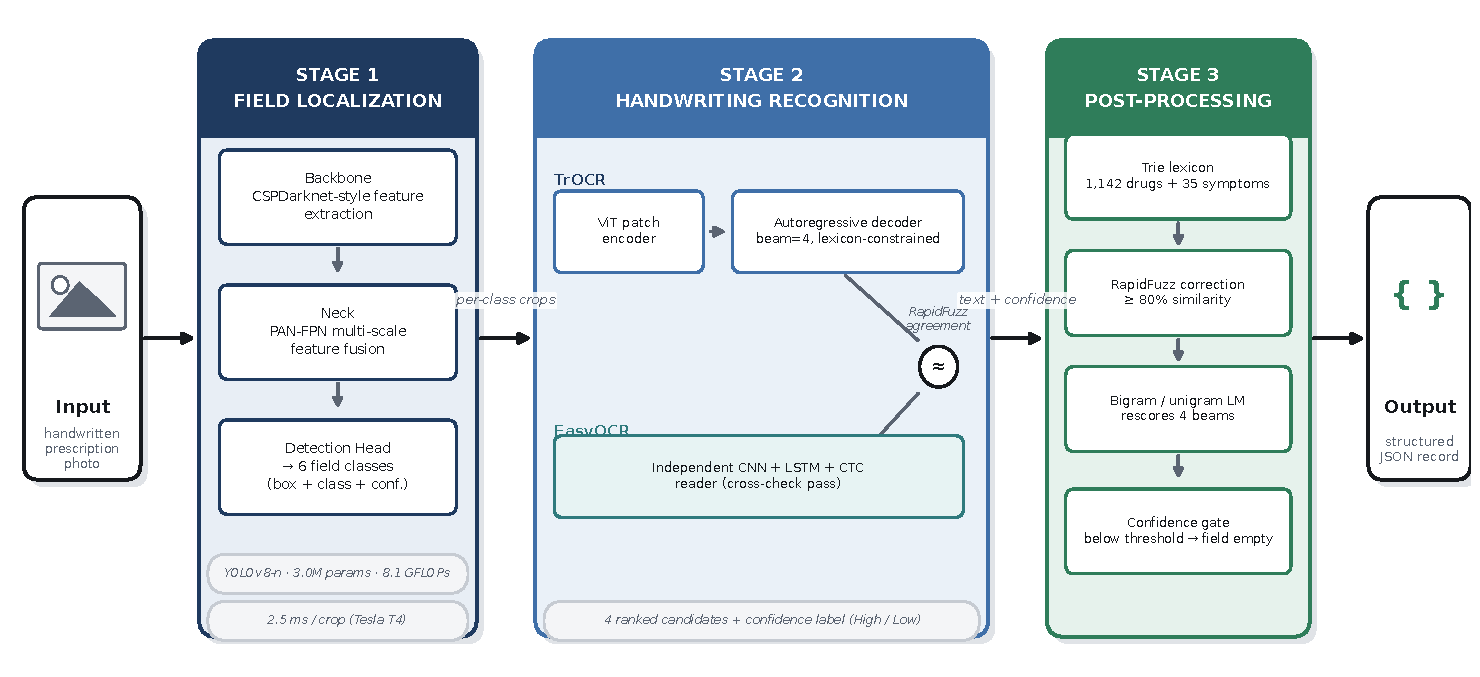
\includegraphics[width=\linewidth]{figures/model_block_diagram.pdf}
  \caption{Medi-Script-AI complete architecture. Each stage is a specialist model with its own internal structure, not a single monolithic network: Stage~1 (YOLOv8-nano) localizes six field classes; Stage~2 pairs TrOCR's constrained-decoding transformer with an independent EasyOCR cross-check, reconciled by RapidFuzz agreement; Stage~3 verifies and corrects the result against domain knowledge before it becomes a structured record. Gray chips report measured operating statistics for each stage.}
  \label{fig:pipeline}
\end{figure*}

\subsection{Stage 1: Field Localization with YOLOv8}
\label{sec:stage1}

We fine-tune a \textbf{YOLOv8-nano} model -- the smallest and fastest variant in the YOLOv8 family~\cite{jocher2023yolov8} -- to detect and localize six distinct field classes, listed in Table~\ref{tab:yolo-classes}.

\begin{table}[t]
  \centering
  \caption{Target field-localization schema.}
  \label{tab:yolo-classes}
  \begin{tabular}{ll}
    \toprule
    \textbf{Class} & \textbf{Description} \\
    \midrule
    \texttt{name}     & Patient's full name \\
    \texttt{age}      & Patient's age \\
    \texttt{gender}   & Patient's gender (M/F) \\
    \texttt{symptoms} & Presenting complaints \\
    \texttt{medicine} & Prescribed drug name(s) \\
    \texttt{dosage}   & Drug dosage and frequency \\
    \bottomrule
  \end{tabular}
\end{table}

\textbf{Why YOLOv8-nano?} At 3.0M parameters and 8.1 GFLOPs, the nano variant is the smallest architecture in the YOLOv8 family and is, in principle, compact enough to run on constrained edge hardware such as a Raspberry Pi -- a prerequisite for deployment in rural clinics without GPU infrastructure. Our own benchmark (\S\ref{sec:results}) measured 2.5\,ms per crop on a single Tesla~T4 GPU; we have not yet separately profiled genuine CPU-only inference on target edge hardware, and we treat that as an open measurement rather than assume it from the model's parameter count alone (\S\ref{sec:temporal-coupling}).

\textbf{Training.} For the medicine-only prototype reported in this paper, we trained for 50 epochs on the Bannari Amman Institute of Technology handwriting dataset~\cite{bannari2023handwritten}. Results are reported in \S\ref{sec:results}. The full six-class model requires annotating real-world Indian prescription images, which is in progress and described as Phase~2 of our future work (\S\ref{sec:future-work}).

\subsection{Stage 2: Handwriting Recognition with TrOCR}
\label{sec:stage2}

Each bounding box detected by YOLO is cropped from the original image and passed to Microsoft's \textbf{TrOCR} (\texttt{trocr-base-handwritten})~\cite{li2023trocr}, a Transformer-based model that encodes the image patch with a ViT encoder and decodes it token-by-token with a BERT-style decoder.

We use beam-search decoding with \texttt{num\_beams=4} (four candidate sequences per crop, all four retained for rescoring), \texttt{no\_repeat\_ngram\_size=3} to prevent repetition, and a \texttt{prefix\_allowed\_tokens\_fn} constraint that, for the \texttt{medicine} field, restricts the decoder to token sequences that are valid continuations of known drug names in our medical lexicon -- a form of constrained decoding. The four beam candidates are then rescored by our domain language model (\S\ref{sec:stage3}).

\textbf{Cross-validation with EasyOCR.} TrOCR's output for each crop is independently cross-checked against an EasyOCR prediction. If both models agree (RapidFuzz ratio $>$ 85\%), confidence is elevated to ``High.'' If they disagree, the lexicon is used as a tiebreaker.

\subsection{Stage 3: Post-Processing with Domain Knowledge}
\label{sec:stage3}

\textbf{Medical lexicon.} We compiled a curated lexicon of 1{,}142 medicines and 35 common symptoms sourced from public drug databases and medical reference materials, stored in a trie for $O(k)$ prefix lookup, where $k$ is the length of the query string.

\textbf{Fuzzy correction.} Raw OCR output is compared against the lexicon using RapidFuzz partial-ratio matching. If the recognized text has a fuzzy-similarity score above 80\% against a known drug name, it is automatically corrected to the canonical name (e.g., \texttt{"paracetamoi"} $\to$ \texttt{"Paracetamol"}). Output that does not clear this threshold against any lexicon entry is left uncorrected rather than forced to the nearest match, which is the behavior that produces the ``safe failure'' outcome discussed in \S\ref{sec:results}.

\textbf{Domain language-model rescoring.} A lightweight bigram/unigram language model trained on medical text rescores the four beam candidates from Stage~2, selecting the candidate with the highest combined acoustic (TrOCR confidence) and linguistic (LM) score.

% =====================================================================
\section{Challenges}
\label{sec:challenges}

\subsection{Data Scarcity and the Annotation Bottleneck}

The single most critical challenge is the absence of a large-scale, publicly available dataset of \emph{real-world} handwritten prescription images with \emph{field-level} bounding-box annotations. Most prior work uses either printed prescription datasets (trivially easy, not representative) or fully synthetic datasets (digitally generated with fonts that resemble nothing like a doctor's cursive handwriting). Creating our own dataset of 500+ annotated real-world Indian prescriptions would take substantial human effort; we are currently building a 44-image seed dataset to bootstrap the training process, which is insufficient on its own for a highly generalizable model.

\subsection{Extreme Handwriting Variability}

Unlike bank cheques or postal forms, medical prescriptions have no mandated handwriting style. Handwriting quality for a single field (``medicine'') ranges from perfectly legible printing to near-indecipherable cursive abbreviation. A model that performs well on one doctor's handwriting may fail completely on another's without substantial training-data diversity.

\subsection{Out-of-Vocabulary Medical Terminology}
\label{sec:oov}

Generic language models assign near-zero probability to medical terms such as ``Azithromycin,'' ``Dexamethasone,'' or ``Atorvastatin.'' Standard beam search, which relies on language-model priors, will therefore actively work \emph{against} correct recognition of these terms -- and, as we show in \S\ref{sec:results}, can instead steer the decoder toward a fluent but entirely unrelated word it considers more probable. Our constrained-decoding approach (\S\ref{sec:stage2}) addresses this but requires a comprehensive lexicon, which is itself hard to keep current as new drugs are approved.

\subsection{YOLO--TrOCR Temporal Coupling}
\label{sec:temporal-coupling}

In our current pipeline, TrOCR runs sequentially on each detected crop. For a prescription with six fields (name, age, gender, symptoms, three medicine lines, dosage), this means up to ten separate TrOCR inference calls; on CPU, each call with \texttt{num\_beams=4} takes approximately 15--30 seconds. The full pipeline can therefore take 2--5 minutes on a laptop CPU -- far too slow for clinical use. A GPU is essentially required for production-speed TrOCR inference, but our target users (small clinics, rural health posts) rarely have GPU infrastructure; this is the same CPU-availability gap noted for Stage~1 in \S\ref{sec:stage1}, and it is substantially more severe here.

\subsection{Image Quality and Perspective Distortion}
\label{sec:image-quality}

In practice, prescriptions are photographed with mobile phones under poor lighting, at angles, or while partially folded. Our pipeline currently assumes a reasonably flat, front-facing image. Significant perspective distortion shifts YOLO's bounding-box predictions, and the resulting crops may contain partial fields or the wrong region entirely. A preprocessing stage for perspective correction and adaptive binarization is needed but not yet implemented.

\subsection{Absence of a Standardized Evaluation Benchmark}

There is no standardized benchmark dataset for Indian medical-prescription parsing, which makes it impossible to compare our system against prior work on common footing. We are forced to evaluate on our own held-out test set, which limits the generalizability of our accuracy claims.

% =====================================================================
\section{Preliminary Results and Error Analysis}
\label{sec:results}

This section reports three things in turn: the quantitative performance of the Stage~1 detector; a comparison against the synthetic-data-trained Donut baseline discussed in \S\ref{sec:related-donut}; and, because neither of these establishes that the full pipeline works end to end, a qualitative case-study analysis of what happens when all three stages run together on real images.

\subsection{Field Localization: Quantitative Results}
\label{sec:quant-results}

We evaluate the Stage~1 detector on the medicine-only prototype described in \S\ref{sec:stage1}: YOLOv8-nano fine-tuned for 50 epochs on the Bannari Amman handwriting dataset~\cite{bannari2023handwritten}. Table~\ref{tab:yolo-results} and Figure~\ref{fig:results} summarize the outcome.

\begin{table}[t]
  \centering
  \caption{YOLOv8-nano medicine-field detection results, medicine-only prototype, 50 epochs. The Donut baseline (\S\ref{sec:baseline}) is reported separately in prose, since it is a qualitative outcome rather than a comparable metric.}
  \label{tab:yolo-results}
  \begin{tabular}{lr}
    \toprule
    \textbf{Metric} & \textbf{Value} \\
    \midrule
    mAP50                                & 86.1\% \\
    mAP50-95                             & 46.2\% \\
    Precision                            & 81.9\% \\
    Recall                               & 80.6\% \\
    Training time (Tesla T4, 50 epochs)  & $\sim$4 min (0.067 GPU-h) \\
    Model size (\texttt{best.pt})        & 6.2 MB \\
    Inference speed (Tesla T4 GPU)       & 2.5 ms / image \\
    \bottomrule
  \end{tabular}
\end{table}

\begin{figure}[t]
  \centering
  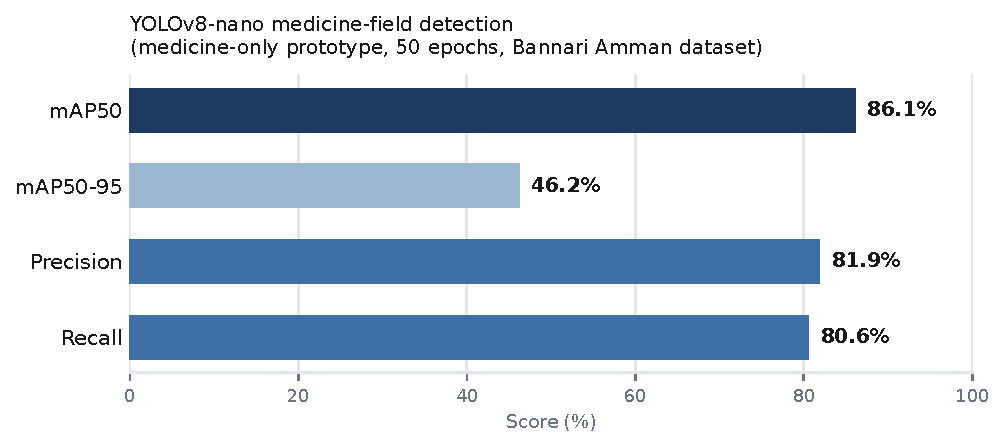
\includegraphics[width=\linewidth]{figures/results_metrics.pdf}
  \caption{YOLOv8-nano medicine-field detection metrics for the medicine-only prototype.}
  \label{fig:results}
\end{figure}

The detector reaches 86.1\% mAP50 and 46.2\% mAP50-95 -- a substantial gap between the two metrics that is typical of handwriting-region detection, where a box is often correctly placed but imprecisely sized around cursive strokes that bleed past the field's nominal boundary. Training converged in approximately four minutes (0.067 GPU-hours) on a single Tesla~T4, and the resulting checkpoint is 6.2\,MB, small enough to distribute to edge devices without a dedicated model-serving pipeline. We measured 2.5\,ms per crop for inference on the same GPU; as noted in \S\ref{sec:stage1}, we have not yet separately benchmarked CPU-only inference on the Raspberry-Pi-class hardware we ultimately target, and we flag this as an open measurement rather than assume it from the model's small parameter count.

Two caveats matter for interpreting these numbers correctly. First, this evaluation covers a single class (\texttt{medicine}); the six-class schema in Table~\ref{tab:yolo-classes} is the target design, not yet the evaluated one -- expanding to all six fields is Phase~2 of our future work (\S\ref{sec:future-work}). Second, the underlying dataset's annotations are coarse: bounding boxes were drawn around medicine lines without consistently correcting for overlap or omission. We believe this is the direct cause of Recall trailing Precision, and that better-curated annotations, not additional training epochs, are the more promising lever for improving this stage further.

\subsection{Baseline Comparison: Synthetic-to-Real Transfer Failure}
\label{sec:baseline}

To situate this result against the alternative architecture discussed in \S\ref{sec:related-donut}, we ran the pretrained Donut checkpoint associated with the \texttt{chinmays18/medical-prescription-dataset}~\cite{shrivastava2024medocr} -- fine-tuned entirely on synthetic, digitally rendered prescription images -- directly on a real, photographed hospital prescription. The model produced no usable output: its decoder emitted a repeating sequence of period characters (\texttt{". . . . . . ."}) regardless of the input's actual content, indicating that the synthetic-to-real domain gap here is severe enough to collapse the output distribution entirely rather than merely degrade accuracy. This is consistent with the broader pattern in \S\ref{sec:related-donut}: end-to-end document-understanding transformers pretrained or fine-tuned on synthetic layouts transfer poorly to the visual statistics of real handwriting, regardless of how capable they are on in-domain benchmarks.

\subsection{End-to-End Pipeline: Qualitative Case Studies}
\label{sec:case-studies}

Detector accuracy and a failed baseline comparison do not, on their own, establish that the full YOLO~$\to$~TrOCR~$\to$~lexicon pipeline works end to end. We therefore report two case studies from our own integration testing that were, initially, disappointing -- and that we believe are more informative at this stage of the project than a single aggregate accuracy number would be.

\textbf{Case study A: in-distribution image.} We ran the full pipeline on a held-out test image from the same Bannari Amman distribution used for training, so any failure here cannot be attributed to a train/test domain shift. Stage~1 performed as expected: YOLO correctly localized four separate medicine-line bounding boxes. Stage~2 did not. TrOCR's raw transcriptions for these four crops -- for example \texttt{"wrapportingly ."} and \texttt{"pur-todac itself"} -- are not near-misses on the true drug names; they are not lexical items in any language, at confidence scores of 32.5--53.8\%. Because these scores fall below the fuzzy-matching threshold described in \S\ref{sec:stage3}, Stage~3 correctly declined to force a lexicon correction on any of the four fields, and the pipeline returned an empty \texttt{prescription} field rather than a fabricated one. We read this as a partial validation of the confidence-gated design: the system failed \emph{safely} rather than silently returning a wrong drug name, which for a medical application is the more important of the two properties. It is nonetheless still a failure to extract the record, and it isolates the fault specifically to Stage~2 -- Stage~1's boxes and Stage~3's rejection logic both behaved correctly.

\textbf{Case study B: out-of-distribution image.} We repeated the test on a real hospital prescription photographed independently of any dataset used in training; Figure~\ref{fig:detection-example} shows the original photograph alongside Stage~1's output on it. Stage~1 again localized a medicine field correctly, but Stage~2 produced a different and more concerning failure mode: instead of low-confidence noise, TrOCR returned a fluent, high-confidence transcription of a real, unrelated commercial product name that did not appear anywhere on the page. This is the failure mode anticipated in \S\ref{sec:oov}: when the true handwriting is illegible to the decoder, its language-model prior -- trained on general text, not clinical vocabulary -- gravitates toward whatever plausible-looking string is nearest in its own distribution rather than abstaining. A fluent wrong answer is more dangerous than an obvious one, because it is more likely to pass a rushed human review unchallenged. This example is the clearest evidence in our testing for why constrained decoding and lexicon verification (\S\ref{sec:stage3}) are necessary components of the pipeline rather than optional refinements.

\begin{figure}[t]
  \centering
  \begin{subfigure}[b]{0.48\linewidth}
    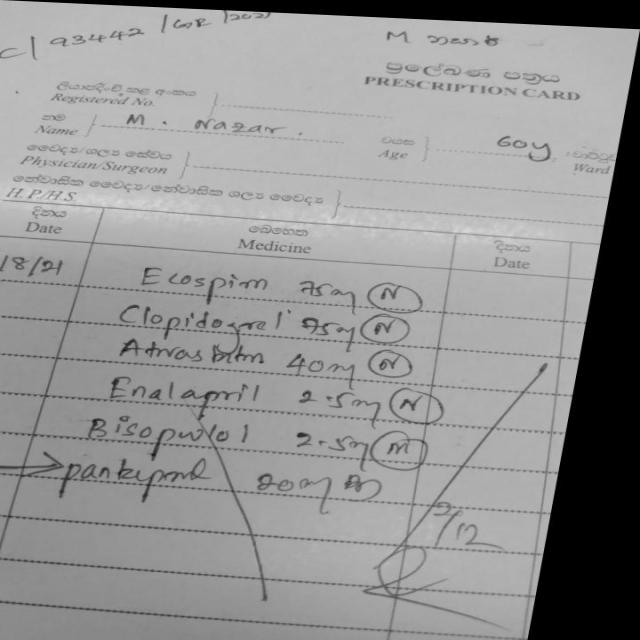
\includegraphics[width=\linewidth]{figures/og_presc.jpg}
    \caption{Original photograph}
    \label{fig:og-presc}
  \end{subfigure}
  \hfill
  \begin{subfigure}[b]{0.48\linewidth}
    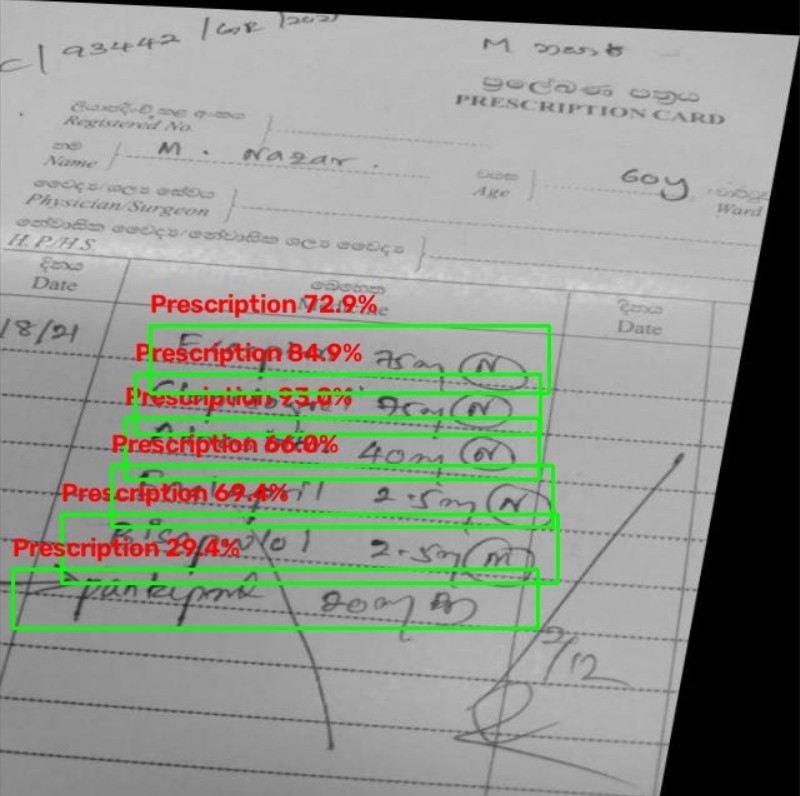
\includegraphics[width=\linewidth]{figures/yolo_presc.jpg}
    \caption{Stage~1 output}
    \label{fig:yolo-presc}
  \end{subfigure}
  \caption{The out-of-distribution image from case study B. (a) the real hospital prescription as photographed, independent of any training data; (b) the same image after Stage~1, with YOLOv8-nano's bounding box drawn around the medicine line. Localization is correct here -- the box tightly bounds the handwritten drug name -- which isolates the fault in this case to Stage~2's transcription of that crop, the fluent hallucination described in the text.}
  \label{fig:detection-example}
\end{figure}

A methodological note from the same test run is worth recording for other groups building similar multi-stage pipelines. An early version of this run appeared to correctly extract the patient's name field, which briefly looked like a partial pipeline success. Closer inspection traced this to a configuration fault that silently routed the image through a legacy flat-OCR-plus-rule-based-parser fallback (\S\ref{sec:generic-ocr}) rather than through YOLO and TrOCR at all; the name was recovered only because the hospital pad happened to pre-print a ``Name:'' label that the flat OCR pass could read cleanly, not because the proposed architecture succeeded. We record this because it is a general risk in multi-path pipeline systems: without per-stage provenance logging, a fallback path's success can be mistaken for the primary path's success. All results reported in this paper have since been re-verified against explicit path-level logs.

% =====================================================================
\section{Conclusion and Future Work}
\label{sec:conclusion}

Medi-Script-AI separates prescription digitization into two specialist problems -- where the information is, and what it says -- on the premise that a single, generic document-understanding model is not well suited to either. Our results partially support this premise and partially complicate it. The localization half holds up: a YOLOv8-nano detector, fine-tuned for a few minutes on a small and imperfectly annotated real-world dataset, reliably finds prescription fields (86.1\% mAP50), on hardware modest enough for edge deployment. The recognition half does not yet hold up, and our case studies in \S\ref{sec:case-studies} show two distinct ways it fails: as low-confidence noise that a lexicon gate can safely reject (case study A), and, more seriously, as fluent, high-confidence hallucination produced by language-model priors when handwriting is genuinely illegible to a general-purpose OCR model (case study B). Both failures trace to the same root cause -- \texttt{trocr-base-handwritten} was never trained on clinical handwriting or drug vocabulary -- and neither is fixed by improving Stage~1 or Stage~3.

We draw three specific, evidence-motivated conclusions. First, generic pretrained handwriting OCR, not only synthetic-data-trained document-understanding models, fails on real clinical handwriting: the domain gap is not only synthetic-vs-real, as the Donut baseline alone would suggest, but also general-handwriting-vs-clinical-handwriting. Second, a confidence-gated, lexicon-aware post-processing stage is not a refinement but a safety-relevant necessity, since it is the only component in our current pipeline that reliably distinguishes ``the model does not know'' from ``the model is confidently wrong.'' Third, the path to a working system runs specifically through Stage~2, and we already have the pieces in place to pursue it.

\subsection{Future Work}
\label{sec:future-work}

We plan to close this gap in three phases.

\textit{Phase 1 -- Fine-tune TrOCR on real handwriting.} We will label 200--300 crops sampled directly from YOLO's own detections on real prescriptions with their correct text, and fine-tune \texttt{trocr-base-handwritten} on these pairs. Our training script is already implemented; at 10--20 epochs on a single Colab T4 GPU, each fine-tuning run costs under 30 minutes, making this the fastest-to-test item in the plan.

\textit{Phase 2 -- Expand YOLO to all six fields.} We will annotate approximately 100 real prescription images across the \texttt{name}, \texttt{age}, \texttt{gender}, \texttt{symptoms}, \texttt{medicine}, and \texttt{dosage} classes and retrain the detector on the full schema in Table~\ref{tab:yolo-classes}, targeting $>$85\% mAP50 across all classes based on the medicine-only result in \S\ref{sec:quant-results}.

\textit{Phase 3 -- End-to-end validation on held-out prescriptions.} Once both models are updated, we will evaluate the complete pipeline on prescriptions excluded from either training set, reporting both per-field accuracy and exact-record-match accuracy, and repeat the case-study analysis of \S\ref{sec:case-studies} to confirm the hallucination failure mode is actually resolved rather than merely less frequent.

Longer term, we plan to add a perspective-correction and adaptive-binarization preprocessing stage for images taken at an angle or under poor lighting (\S\ref{sec:image-quality}), extend the lexicon and language model to Hindi, Tamil, and Kannada drug and patient names, and package the pipeline behind a mobile front end so pharmacists can scan and verify prescriptions in real time.

% =====================================================================
\bibliographystyle{IEEEtran}
\bibliography{references}

\end{document}